\chapter{面向异构后端的容器内存压力感知卸载架构设计与实现}

本章详细介绍了面向容器环境的异构分层内存协同卸载系统的设计与实现细节。\ref{sec:基于同步回收延迟的内存压力量化算法的设计与实现} 节介绍了基于同步回收延迟的内存压力量化算法的设计与实现,首先分析了同步回收延迟与内存压力的关联性,然后提出了基于同步回收延迟的内存压力量化算法,最后介绍了该算法的实现细节。


\section{基于同步回收延迟的内存压力量化算法的设计与实现}
\label{sec:基于同步回收延迟的内存压力量化算法的设计与实现}
这一章的核心目标是详细阐述基于同步回收延迟的内存压力量化算法的设计思想、具体实现步骤、以及实现中的关键技术细节。

\subsection{同步回收延迟与内存压力的关联分析}

在传统的内存管理研究中,工作集估计算法扮演着重要角色,其准确性直接影响着内存分配、页面置换等关键决策。鉴于工作集估计算法高度依赖于对系统内存压力的准确量化,本节首先深入剖析同步回收延迟与内存压力之间的内在关联。

传统的工作集估计算法,如WSE (Working Set Estimation) 和WSE-Lite,通常依赖于对缺页中断次数、内存分配次数等统计信息的分析来间接推断工作集大小。这些算法需要在内核中维护相应的计数器,并进行周期性的采样,由此引入的CPU开销不容忽视。更为关键的是,这些统计信息与工作集大小之间并非严格的线性关系,而是受到多种因素的复杂影响。例如,在应用程序频繁切换不同工作集时,即使整体工作集规模保持相对稳定,代码和数据的局部性特征也可能导致大量的缺页中断,从而干扰算法对工作集大小的准确判断。此外,随着存储技术的快速发展,现代计算系统越来越多地采用异构存储设备(如不同类型的SSD、NVMe等)作为后端存储。然而,许多现有的工作集估计算法在设计时并未充分考虑这些异构存储设备在性能上的显著差异,这可能导致算法在不同存储后端上的表现出现较大偏差,进而影响系统整体的内存管理效率。

为了克服上述局限性,本研究提出了一种基于内存压力的工作集估计算法,其核心思想根植于Linux内核广泛采用的同步内存回收机制。当容器的内存使用量逼近其cgroup资源限制时,内核会主动触发同步内存回收,尝试将部分不活跃的冷页面装卸到异构设备上,以释放内存空间。同步内存回收过程所消耗的时间,即同步回收延迟,构成了衡量系统内存压力的一个关键指标。这种关联性源于内存回收机制的内在逻辑:在系统内存资源充裕的情况下,通常不存在显著的内存压力,同步回收机制很少被触发,因此延迟极低。反之,当系统面临内存压力时,即内存资源趋于紧张,同步回收过程需要花费更多的CPU时间片来扫描和选择合适的页面进行换出,从而导致同步回收延迟显著增加。因此,通过精确监测同步回收延迟,我们能够敏锐地捕捉到系统内存压力的动态变化。与传统的基于统计信息的方法相比,我们的算法直接监测同步回收事件本身并记录其延迟。这种设计带来了多方面的显著优势:首先,同步回收延迟作为内存压力的直接体现,与工作集大小具有更强的内在关联性,能够更准确地反映工作集的变化趋势;其次,由于仅在同步回收事件发生时才进行数据采集,避免了持续性的统计信息收集与处理,从而显著降低了CPU开销;此外,同步回收延迟本身内在地整合了后端存储设备的性能因素,不同存储设备的性能差异自然地反映在同步回收延迟的长短上,使得我们的算法能够天然地适应异构存储环境,无需额外的配置或参数调整;最后,这种设计将底层异构存储的具体实现细节进行了抽象,算法层面仅关注同步回收所需的时间,从而简化了算法的设计并提高了其通用性和可移植性。

\subsection{基于同步回收延迟的内存压力监测与量化算法}
\label{sec:基于同步回收延迟的内存压力监测与量化算法}

在 \ref{sec:直接页面回收机制} 节中,我们对 Linux 内核直接页面回收机制做了详细的分析,分析表明,函数\_\_alloc\_pages\_direct\_reclaim 的执行时间是反映同步回收延迟的重要指标。基于此,本章提出了一种内存压力检测方法。该方法利用内核插桩技术,在 \_\_alloc\_pages\_direct\_reclaim 函数的入口和出口处记录时间戳,从而直接获取每次同步回收操作的耗时。为了综合反映多 CPU 系统中不同核心的负载差异,我们引入了多 CPU 加权聚合策略。此外,为了平滑压力数据、减少短期波动的影响,我们采用了指数移动平均算法。最终,该方法将内存压力以百分比的形式输出到用户空间,为应用程序和系统管理员提供了一种轻量级、响应及时的内存压力监控手段。

\subsubsection{多核加权聚合}

我们通过插桩技术得到是单个核心的同步回收延迟时间 \(T_c^{block}\),我们需要将多个核心的 \(T_c^{block}\) 聚合为一个压力值。然而,采用简单的算术平均方法计算系统压力:
\begin{equation}
    Pressure_{simple} = \frac{\sum_{c=1}^{n} T_c^{block}}{\Delta T \times n} \times 100\%
\end{equation}

其中,\(\Delta T\) 为采样周期,\(n\) 为处理器核心数量,该方法存在显著的理论缺陷,无法准确反映系统的真实内存压力状况。

首先,简单平均算法未能有效处理处理器核心负载不均衡问题。考虑一个多核系统,其中部分处理器核心处于高负载状态,而另一些核心处于空闲或低负载状态。当空闲核心上发生短暂的同步内存回收事件时,其对应的  也会被计入总和。例如,在一个四核系统中,假设一个高负载核心因内存压力产生了 0.5s 的阻塞时间,而一个空闲核心仅因参与全局同步产生了 0.1s 的阻塞时间。根据简单平均算法,系统压力将被计算为:

\[
Pressure_{simple} = \frac{0.5 + 0.1 + 0 + 0}{1.0 \times 4} \times 100\% = 15\%
\]

该结果显著低估了实际系统压力,因为将空闲核心的数据纳入计算,稀释了高负载核心所反映的真实内存压力。这种现象可定义为"空闲核心稀释效应",导致系统压力评估结果失真。

其次,简单平均算法无法准确反映不同处理器核心对系统整体性能的差异性贡献。在实际系统中,各处理器核心的负载分布往往呈现显著差异,部分核心可能长时间处于高负载状态,而其他核心则可能大部分时间处于空闲状态。简单平均算法平等对待每个核心的延迟时间,忽略了它们对系统整体性能影响的权重差异。例如,在一个双核系统中,若核心0的压力为 80\%(非空闲时间 80ms),核心1的压力为 20\%(非空闲时间 20ms),简单平均算法将得出 50\% 的系统压力。该结果未能体现核心0作为主要负载承担者的关键作用。

为克服上述缺陷,本研究提出采用加权聚合算法,该算法的核心思想是:根据每个处理器核心的运行时间分配权重。核心的运行时间越长,表明其在采样周期内处理的任务越多,其上发生的同步内存回收事件对系统整体性能的影响也越显著,他的行为也更具有代表性。 加权聚合算法的计算公式如下:

\begin{equation}
    Pressure_{weighted} = \frac{\sum_{c=1}^{n} (T_c^{block} \times W_c)}{\sum_{c=1}^{n} W_c \times \Delta T} \times 100\%
\end{equation}

其中,\(T_c^{block}\) 表示核心 \(c\) 在采样周期 \(\Delta T\) 内的同步内存回收总延迟时间,\(W_c\) 表示核心 \(c\) 的权重,即其在采样周期 \(\Delta T\) 内的非空闲时间。分母中的 \(\sum_{c=1}^{n} W_c\) 等于 \(\Delta T \times n\),表示所有核心的非空闲时间总和。通过这种加权方式,算法能够有效降低或消除空闲核心的"噪声"影响,同时更准确地反映不同核心负载对系统整体性能压力的贡献,从而提供更可靠、更具代表性的内存压力评估结果。

\subsubsection{指数移动平均算法}

在获取基于处理器核心的非空闲时间加权的内存压力指标后,我们还需要进一步考虑压力数据的平滑性以及长期趋势的分析。原始的压力数据(无论是简单平均还是加权平均)可能会因为短暂的、偶然的事件而产生剧烈波动,这些波动可能会掩盖真实的压力趋势。因此,需要采用一种有效的方法对压力数据进行平滑处理,以减少短期波动的影响,同时保留长期趋势信息。指数移动平均(Exponential Moving Average, EMA)算法是满足这一需求的有效工具。

EMA 算法的核心思想是对新旧数据进行加权平均,但与简单算术平均赋予所有数据相同权重不同,EMA 赋予旧数据的影响随时间推移呈指数衰减。这种处理方式更符合实际系统的运行特征:最近发生的事件对当前系统状态的影响通常更大,而较早发生的事件的影响则逐渐减弱。具体来说,EMA 的计算公式为:
\begin{equation}
    EMA_{new} = EMA_{old} \times \alpha + P_{current} \times (1 - \alpha)
    \label{eq:EMA}
\end{equation}


其中,\(EMA_{new}\) 和 \(EMA_{old}\) 分别代表当前时刻和上一时刻的 EMA 值,\(P_{current}\) 是当前时刻的压力值,\(\alpha\) 是一个介于 0 和 1 之间的衰减因子(也称平滑因子)。衰减因子 \(\alpha\) 决定了旧数据影响力衰减的速度,也即决定了 EMA 对历史数据的"记忆"长度。它的值由采样间隔 \(\Delta T\) 和时间窗口 \(\tau\) 共同决定,关系式为:
\[
\alpha = e^{-\Delta T / \tau}
\]

其中,\(\Delta T\) 是采集内存压力数据的频率(例如,每 2 秒采样一次),\(\tau\) 则反映了希望 EMA 追踪的压力趋势的时间尺度(例如,10 秒、60 秒或 300 秒)。\(\tau\) 越大,\(\alpha\) 越小,EMA 曲线越平滑,对短期波动的抑制能力越强,但对真实压力变化的反应也越迟钝;反之,\(\tau\) 越小,\(\alpha\) 越大,EMA 曲线对新数据的响应越灵敏,但平滑效果也越差。

相比于简单平均或固定窗口的移动平均算法,EMA 算法具有显著优势。首先,EMA 算法的计算非常高效。它仅需存储上一时刻的 EMA 值,无需维护一个包含大量历史数据的窗口,计算复杂度为 \(O(1)\)。这使得 EMA 非常适合于资源受限的嵌入式系统或需要高频采样的实时监控系统。其次,EMA 算法的参数可调性提供了极大的灵活性。通过调整衰减因子(即调整时间窗口),可以在快速响应和数据平滑之间找到最佳平衡点。这使得 EMA 能够适应不同的应用场景和性能需求。最后,也是最重要的一点,EMA 算法能够有效地追踪压力数据的长期趋势。它不仅能平滑短期波动,还能清晰地展现压力随时间变化的整体走向,帮助及时发现潜在的性能瓶颈或系统异常。

虽然 EMA 和平滑前的加权算法都使用了"加权"一词,但需要注意它们含义和目的不同。加权算法基于处理器核心非空闲时间,旨在更准确地衡量当前时刻的平均压力;而 EMA 的加权则是为了在时间维度上平滑压力数据,其核心目标是揭示压力变化的趋势,而非单纯的平均值计算。

\subsubsection{定点数优化}
\label{sec:fixed_point_optimization}

在实时监控和评估系统内存压力的过程中,频繁的数值计算是不可避免的。特别是在计算内存压力指标以及进行 EMA 平滑处理时,会涉及到大量的浮点数运算。虽然浮点数能够提供较高的数值精度,但在我们关注的内存压力评估场景中,对计算精度的要求并非绝对的,过高的精度反而可能导致不必要的计算资源浪费。因此,我们引入定点数表示法,旨在保证足够精度的前提下,显著提升计算效率。定点数的核心思想在于,通过一个预先确定的缩放因子将实数映射为整数进行存储和运算,从而避免浮点运算。与浮点数动态调整小数点位置不同,定点数的小数点位置是固定的。对于任意实数 \(R\),其定点数表示 \(D\) 可以定义为:

\[
D = \lfloor R \times F \rfloor
\]

其中,\(F\) 表示缩放因子,\(\lfloor \cdot \rfloor\) 表示向下取整操作。为了能够利用计算机底层高效的位移操作来实现乘除运算,缩放因子 \(F\) 通常选择 2 的整数次幂形式,即 \(F = 2^n\)。在本文的应用场景中,我们选择 \(F = 2^{10} = 1024\) 作为缩放因子。这一选择在计算精度和效率之间取得了较好的平衡。

对于任意实数 \(R\), 其定点数表示 \(D\) 会引入量化误差. 量化误差定义为实数与其定点数表示之间的差值:
\[
\epsilon = R - \frac{D}{2^{10}}
\]
由于 \(D\) 是 \(R \times 2^{10}\) 的向下取整结果, 因此存在一个非负实数 \(\delta\)(且 \(\delta < 1\)), 使得:
\[
R \times 2^{10} = D + \delta
\]
将上式两边同时除以 \(2^{10}\), 得到:
\[
R = \frac{D}{2^{10}} + \frac{\delta}{2^{10}}
\]
将此表达式代入量化误差的定义式, 得到:
\[
\epsilon = \frac{\delta}{2^{10}}
\]
由于 \(0 \leq \delta < 1\), 因此量化误差 \(\epsilon\) 满足:
\[
0 \leq \epsilon < 2^{-10} \approx 0.000977
\]
选择\(2^{10}\)作为缩放因子,定点数表示的量化步长为\(2^{-10} \approx 0.000977\)。这意味着对于任意值\(v\),其定点数表示的:最大绝对误差:\(< 0.000977\); 相对误差:\(< 0.000977/v\)。

在定点数的运算过程中,除了量化误差外,还会引入运算误差。假设有两个实数 \(R_1\) 和 \(R_2\), 它们对应的定点数表示分别为 \(D_1\) 和 \(D_2\). 进行加法(或减法)运算时,实际计算的是定点数的和(或差),然后再将结果转换回实数域:
\[
(R_1 \pm R_2) - \frac{D_1 \pm D_2}{2^{10}}
\]
由于\(D_1\)和\(D_2\)的计算都存在误差,且\(0 \leq \epsilon < 2^{-10} \approx 0.000977\),所以
\[
|(R_1 \pm R_2) - \frac{D_1 \pm D_2}{2^{10}}| < 2 \times 2^{-10}
\]

对于两个实数的乘法 \(R_1 \times R_2\), 在定点数运算中, 我们首先计算两个定点数的乘积 \(D_1 \times D_2\), 然后为了保持正确的缩放, 需要将结果右移 10 位(相当于除以 \(2^{10}\)):
\[
(D_1 \times D_2) >> 10
\]
这一操作可以等效为:
\[
(D_1 \times D_2) >> 10 = (R_1 \times R_2) \times 2^{10} + \epsilon_{mul}
\]
其中乘法误差 \(|\epsilon_{mul}| < 2^{-9} + R_1\epsilon_2 + R_2\epsilon_1\)。

在内存压力计算的具体应用中,我们可以采用定点数来替代浮点数进行运算。以 EMA 平滑为例,原始的浮点数计算公式为:
\[
EMA_{new} = EMA_{old} \times \alpha + P_{current} \times (1 - \alpha)
\]

将其转换为定点数形式:
\[
EMA_{new\_fixed} = (EMA_{old\_fixed} \times \alpha_{fixed} + P_{current\_fixed} \times (F - \alpha_{fixed})) >> 10
\]

其中,\(EMA_{old\_fixed}\)、\(P_{current\_fixed}\) 和 \(\alpha_{fixed}\) 分别是 \(EMA_{old}\)、\(P_{current}\) 和 \(\alpha\) 的定点数表示(即乘以 1024 并向下取整的结果)。通过这种转换,我们将原本的浮点数乘法和加法运算替换为整数乘法、加法和位移运算,在保证足够精度的前提下,显著提高了计算速度。

\subsubsection{时间漂移的处理机制}

在高负载场景下,工作队列可能无法严格按照预定周期执行数据处理任务,导致时间漂移现象的发生。本研究针对时间漂移问题,从数据处理时机和延迟数据处理两个方面展开分析,并提出相应的优化策略。

\paragraph{数据处理时机的校正}
理想情况下,数据处理应在时刻序列
\[
t_0, \quad t_0 + T, \quad t_0 + 2T, \quad t_0 + 3T, \quad \dots
\]
依次执行,其中 \(t_0\) 为初始时刻,\(T\) 为预定周期。然而,实际执行时刻可能因延迟变为
\[
t_0, \quad t_0 + T + \Delta_1, \quad t_0 + 2T + \Delta_1 + \Delta_2, \quad \dots
\]
其中 \(\Delta_i\) 表示第 \(i\) 次执行的延迟时间。

为避免延迟的累积效应,本研究提出基于周期对齐的调度策略。在任务执行完毕后,计算错过的完整周期数:
\[
\text{missed\_periods} = \left\lfloor \frac{\text{now} - \text{expires}}{T} \right\rfloor,
\]
并将下一次执行时间设定为:
\[
\text{next\_update} = \text{expires} + (1 + \text{missed\_periods}) \times T.
\]
该策略确保系统在经历显著延迟后,能够跳过被错过的周期,回归到最接近理想序列的下一个完整节拍,从而有效避免时间漂移的累积效应。

\paragraph{延迟数据的处理}

在多周期(时间漂移)未更新的情况下,生产者端可能持续累积停顿时间数据,但由于工作队列作为消费者未能及时处理,导致单次统计结果可能超过既定周期长度,从而出现超过 100\% 的不合理值。为避免此问题,本研究采用了"截断 + 推迟"的处理策略:当检测到单周期(长度为 \(\textit{period}\))内的累计值超出上限时,不直接丢弃超额部分,而是先将其截断至 \(\textit{period}\),再将"剩余量"保留到下一个周期继续累加。这样既能防止当期报告出现超过 100\% 的不可信结果,又不会漏记真实发生的停滞时间;并且当期被截断的那部分在后续周期会逐步补偿,不会产生误差累积。

对于多周期未更新所导致的更大时间跨度缺口,我们进一步使用基于指数幂运算的加速计算方法。当从时刻 \(t\) 到 \(t+n\) 间无更新发生时,可直接通过指数衰减系数 \(\beta^n\) 来快速推进指数移动平均至最新时刻。

% 具体而言,令 \(\beta = e^{-\frac{T}{\tau}}\) 则连续时间下的衰减过程可离散化为
% \[
% \text{EMA}(t+n) \;=\; \beta^n \,\text{EMA}(t)\;+\; \alpha \,\text{Sample}(t+n),
% \]
具体而言,当在 \(n\) 个周期内未更新时,需要从时刻 \(t\) 推进至时刻 \(t+n\)。为方便表示,令 \(\beta = 1-\alpha\)。则:

\begin{equation}
\text{EMA}(t+2) = \beta \,\text{EMA}(t+1) + \alpha \,\text{Sample}(t+2).
\end{equation}

将 \(\text{EMA}(t+1)\) 展开:

\begin{equation}
\begin{aligned}
\text{EMA}(t+2)
&= \beta \left[\beta\,\text{EMA}(t) + \alpha\,\text{Sample}(t+1)\right] + \alpha\,\text{Sample}(t+2) \\
&= \beta^2 \,\text{EMA}(t) + \beta \alpha\,\text{Sample}(t+1) + \alpha\,\text{Sample}(t+2).
\end{aligned}
\end{equation}

依此类推,若持续展开 \(n\) 步,得到:

\begin{equation}
\text{EMA}(t+n) = \beta^n \,\text{EMA}(t) + \sum_{k=1}^{n} \beta^{\,n-k} \, \alpha \,\text{Sample}(t+k).
\end{equation}

如果仅在最后时刻 \(t+n\) 才获得一个样本 \(\text{Sample}(t+n)\)(而前 \(n-1\) 步样本可视为 0),则上式可简化为:

\begin{equation}
\label{eq:EMA_2}
\text{EMA}(t+n) = \beta^n \,\text{EMA}(t) + \alpha \,\text{Sample}(t+n).
\end{equation}
简化后能显著节省计算量并保持趋势估计的准确性。

\begin{algorithm}[H]
    \caption{内存压力采样漂移的补偿算法}
    \label{alg:mp-drift-compensation}
    \KwIn{\(\textit{memory\_pressure}\):当前内存压力统计对象, \(\textit{period}\):统计周期长度}
    \KwOut{更新后的 \(\textit{memory\_pressure.total\_prev}\),其中超出部分被截断并推迟到后续周期}

    \SetAlgoLined
    \LinesNumbered
    \Begin{
        \(\textit{raw\_sample} \gets \textit{memory\_pressure.total} - \textit{memory\_pressure.total\_prev}\)\;
        \If{\(\textit{raw\_sample} > \textit{period}\)}{
            \(\textit{raw\_sample} \gets \textit{period}\)\;
        }
        \(\textit{memory\_pressure.total\_prev} \gets \textit{memory\_pressure.total\_prev} + \textit{raw\_sample}\)\;
        \tcp{注:\(\textit{memory\_pressure.total}\)中剩余的超量并未丢弃;}
        \tcp{在下一周期的差值计算中会将其补偿。}
    }
\end{algorithm}

% \vspace{3pt}
% \noindent\textbf{算法 \ref{alg:mp-drift-compensation} 解释:}  
% \textit{memory\_pressure.total} 表示自系统启动以来累计的压力(停滞)总量,\textit{memory\_pressure.total\_prev} 为上一次统计后的基准值。第 1 行计算了当期的原始增量 \(\textit{raw\_sample}\)。若该增量超出 \(\textit{period}\),则在第 2--4 行中对其进行截断,防止单周期统计出现超过 100\% 的结果;截断后实际纳入本周期统计的数值记回 \(\textit{memory\_pressure.total\_prev}\),而超额部分仍滞留在 \(\textit{memory\_pressure.total}\) 中,在下一次统计时通过相应的差值计算来纳入。如此策略可避免当期误报高值,并保持长期累积结果与真实压力的吻合。

通过上述处理,本研究在保证计算效率的同时,维持了统计结果的准确性与可解释性。当系统检测到多周期漂移时,可将中间阶段视为零贡献并采用指数衰减对 EMA 快速推进\ref{eq:EMA_2},从而进一步减少计算量并维持整体趋势的合理性,显著提升了内存压力监控的实时性与可靠性。



\subsection{基于同步回收延迟的内存压力监测与量化实现}

在\ref{sec:基于同步回收延迟的内存压力监测与量化算法} 节中,我们阐述了基于同步回收延迟进行内存压力监测的算法原理。在 \ref{sec:容器环境下面向异构装卸后端内存优化框架执行流程} 节中,我们介绍了流程,本节我们介绍实现细节。

\subsubsection{基于生产者-消费者模式的内存压力监测与量化实现}

\begin{figure}[H]
    \centering
    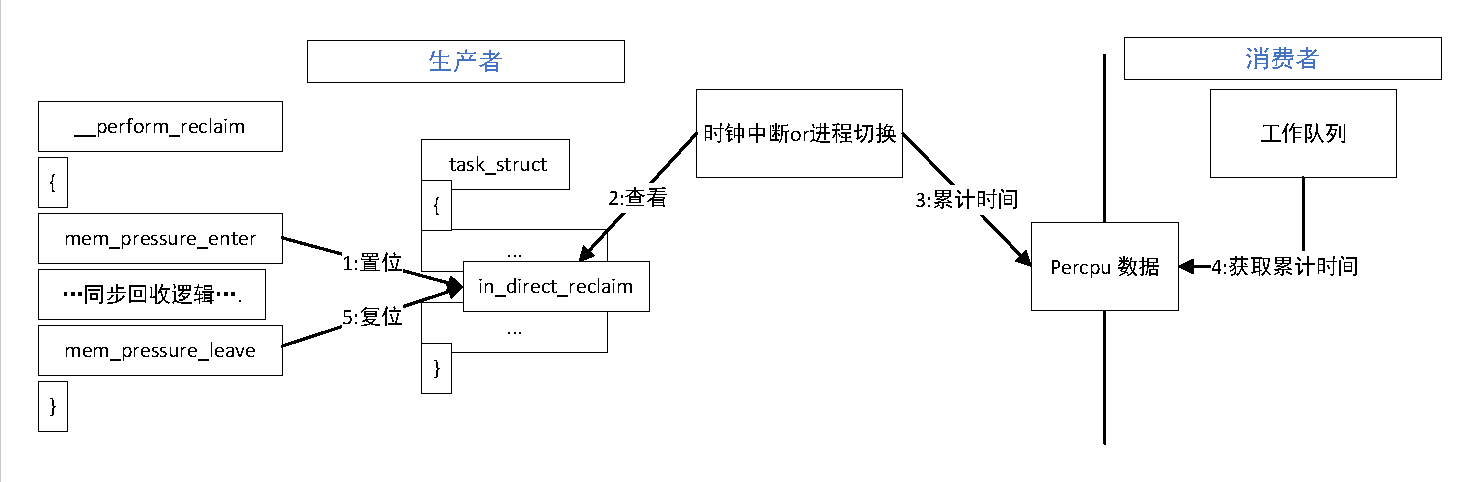
\includegraphics[width=\textwidth]{生产者和消费者.pdf}
    \caption{生产者消费者架构图}
    \label{fig:producer-consumer}
\end{figure}



系统实现采用生产者-消费者模式构建内存压力实时监控与评估框架。该模式通过解耦数据采集与数据处理两个核心功能模块。生产者模块负责采集内存回收过程中的时间片数据,而消费者模块则周期性地处理这些数据,计算并输出内存压力指标。

生产者模块的核心功能是精确捕获内核中与内存回收相关的状态切换时间信息。为实现这一目标,生产者在同步内存回收的起始和结束时刻改变状态。具体而言,当系统发生直接内存回收时,即进程在分配内存时因内存不足而触发同步回收操作,生产者立即改变状态,并记录时间戳,计算累积时间。当同步回收过程结束,进程恢复正常执行时,生产者再次改变状态,并记录时间戳,并计算累积时间。

此外,为确保全面、准确地捕获所有与状态切换相关的时间消耗,生产者在内核调度过程中进行了额外的时间戳记录。具体实现如下:在每次进程调度发生时(即调用 schedule() 函数时),生产者检查当前即将被调度的进程的 task\_struct->  标志。若该标志为 true,表明该进程正处于同步回收状态,即便其即将被调度出去,生产者仍会记录时间戳,以确保其在状态切换上消耗的时间不被遗漏。同时,在每次时钟中断发生时(即 scheduler\_tick() 函数被调用时),生产者检查当前正在运行的进程的 task\_struct->in\_direct\_reclaim 标志。若该标志为 true,表明该进程处于同步回收状态,则记录时间戳,并累加到该 CPU 的每 CPU 变量 direct\_reclaim\_time 中。通过综合同步回收起止事件和内核调度事件的时间戳信息,生产者能够完整地记录所有与状态切换相关的时间消耗。

消费者模块采用工作队列机制实现,其依赖于内核调度器来调度和执行任务。在本系统中,消费者工作队列被配置为每两秒执行一次,其核心任务包括以下四个步骤:

\begin{enumerate}
    \item 数据采集:读取所有 CPU 的 direct\_reclaim\_time 变量的值,这些值代表了在过去两秒内,每个 CPU 上处于同步回收状态的进程所消耗的总时间。
    \item 加权平均计算:将所有 CPU 的同步回收时间进行加权平均,得到整个系统的平均同步回收时间。这一步骤充分考虑了多核系统中各个 CPU 之间的负载均衡情况。
    \item 数据平滑处理:对计算得到的平均同步回收时间应用指数移动平均算法,以消除瞬时波动,准确反映内存压力的长期趋势。
    \item 压力指标计算与输出:根据前文定义的内存压力计算方式,计算得出内存压力值,并判断是否需要通过mpfs通知用户态程序。
\end{enumerate}


\subsubsection{工作队列}
我们最终采用了工作队列来进行内存压力的计算。这主要基于以下几个方面的考虑:内存压力的计算上是一个复杂的统计过程,这个过程需要获取互斥锁并进行较长时间的数据处理。这类操作必须在进程上下文中执行,因为它们可能会引起睡眠,不能在中断上下文中完成。此外,内存压力的监控需要周期性执行以跟踪系统状态的变化,这正好契合工作队列提供的延迟执行机制。而且,由于内存压力的计算主要用于系统监控和决策支持,对实时性要求相对不高,可以容忍一定程度的执行延迟。

工作队列作为Linux内核中经过充分验证的标准机制,为异步任务的执行提供了可靠的保障。它能够确保任务在合适的时机得到执行,并在系统负载较高时自动调节执行频率。特别是对于周期性的监控任务,工作队列实现了完善的补偿机制,即使在系统负载较高导致某些统计周期被延迟时,也能通过计算错过的周期数并进行相应补偿,确保监控数据的连续性和准确性。这种机制对于内存压力监控尤为重要,因为它需要准确反映系统在不同时间段的内存使用状况。

如果采用专用内核线程来实现这些功能,不仅需要手动处理线程的创建、销毁和唤醒,还需要考虑各种边界情况,如系统负载过高时的处理策略、错过统计周期的补偿机制等。这些工作不仅增加了代码的复杂度,也提高了出错的可能性。而在内核编程中,边界条件的处理往往是最容易出现问题的地方,这类问题通常难以重现和调试。相比之下,工作队列已经为这些复杂的情况提供了完善的处理机制,使得开发者可以专注于内存压力计算的核心逻辑实现。

从系统资源利用的角度来看,工作队列的共享特性也带来了显著优势。当系统处于空闲状态时,工作队列中的任务会自动停止,避免不必要的资源消耗;当系统负载升高时,工作队列的调度机制能够自动调节任务的执行频率,确保内存压力监控不会对系统性能造成显著影响。这种自适应的特性,结合工作队列成熟的错误处理机制,为内存压力监控提供了一个稳定可靠的执行环境。


\subsubsection{临界区的保护}

在生产者-消费者模型中,生产者(内存回收路径)负责采集内存回收过程中的时间片数据,而消费者(工作队列)则负责处理这些数据,计算并输出内存压力指标。为了确保数据在并发环境下的完整性和一致性,同时兼顾性能,需要对临界区进行精细的保护。

在详细阐述临界区保护策略之前,简要介绍本文所采用的核心同步机制——序列锁(Seqlock)。序列锁是 Linux 内核提供的一种轻量级同步原语,特别适用于读多写少且写操作简短的场景。其基本原理如图 \ref{fig:seqlock} 所示。序列锁维护一个序列计数器,写操作通过递增该计数器来标识数据更新的开始和结束(奇数表示写操作进行中,偶数表示无写操作)。读操作在开始时记录序列号(\texttt{read\_seqbegin()}),并在读取完成后再次检查序列号(\texttt{read\_seqretry()})。如果序列号发生变化,则表明在读取过程中发生了写操作,读操作需要重试,以确保读取到一致的数据。

\begin{figure}[H]
    \centering
    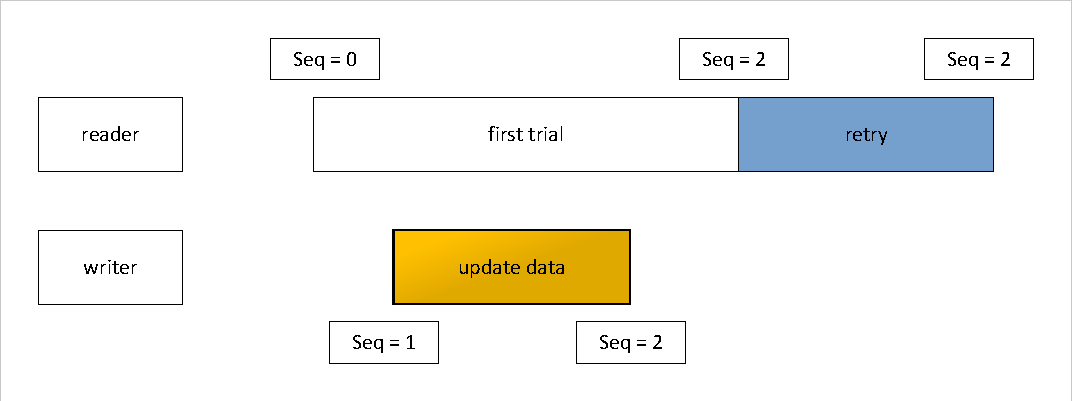
\includegraphics[width=\textwidth]{seqlock.pdf}
    \caption{序列锁(Seqlock)原理示意图}
    \label{fig:seqlock}
\end{figure}

本框架涉及的临界区数据主要包括以下几个方面:

\begin{enumerate}
    \item \textbf{per-CPU 数据:} 每个 CPU 核心维护一份独立的数据结构,用于存储该 CPU 上的累计停顿时间(\texttt{cumulative\_time})和上次统计时间(\texttt{last\_stat\_time})。虽然 per-CPU 变量在更新时本身具有原子性,无需额外加锁,但考虑到消费者需要读取所有 CPU 的 per-CPU 数据进行聚合计算,因此仍需采取适当的同步措施。

    \item \textbf{全局统计信息:} 一个全局静态变量,用于存储所有 CPU 停顿时间的累加值,以及用于平滑计算的历史统计数据。该变量的访问涉及多个 CPU 的数据聚合,因此需要严格的保护。

    \item \textbf{\texttt{task\_struct->in\_direct\_reclaim} 标志:} 进程描述符(\texttt{task\_struct})中的一个标志位,用于标识当前进程是否处于直接内存回收状态。该标志位由生产者(内存回收路径)设置和清除。
\end{enumerate}

基于以上数据结构的特点和访问模式,本框架采用了如下的临界区保护策略:

\begin{itemize}
    \item \textbf{per-CPU 数据中的累计停顿时间(\texttt{cumulative\_time})采用序列锁(Seqlock)保护。}
    \begin{itemize}
        \item 选择序列锁的主要原因是时钟中断处理函数需要更新该数据,而时钟中断处理函数不能阻塞。
        \item per-CPU 数据结构简单,通常为 32 位或 64 位无符号整型,写操作(累加时间)非常快速,且读取时可以整体复制,满足序列锁的使用条件。
        \item 由于内存同步回收通常不是频繁事件,因此对停顿时间的累加操作相对较少,属于典型的读多写少场景,与序列锁的设计理念高度契合。
    \end{itemize}

    \item \textbf{全局统计信息采用互斥锁(Mutex)保护。} 互斥锁提供了更强的互斥性,适用于保护涉及较长时间计算或复杂数据结构的操作。全局统计信息的更新涉及多个 CPU 数据的聚合和历史数据的平滑计算,操作相对耗时,因此采用互斥锁可以确保数据的一致性和完整性。

    \item \textbf{\texttt{task\_struct->in\_direct\_reclaim} 标志的访问由运行队列锁(Runqueue Lock)隐式保护。}
    该标志在同步内存回收开始时置位,在结束时复位。在置位和复位操作期间,内核会持有相应 CPU 的运行队列锁,并关闭本地中断,这可以防止其它 CPU 或中断对当前进程的调度产生干扰。而在时钟中断处理函数中检查该标志时,由于持有运行队列锁可以保证当前进程不会被调度到其它 CPU,因此直接访问该标志是安全的,无需额外的锁保护。这种利用已有锁机制进行保护的方式,避免了引入新的锁,降低了系统的复杂度和开销。
\end{itemize}

通过上述针对性的临界区保护策略,本框架在确保数据一致性的前提下,最大限度地降低了同步开销,提升了系统的整体性能。


\subsubsection{内存压力计算算法}

本节中,算法\ref{alg:helper_functions}和算法\ref{alg:calc_pressure}分别定义了两个核心函数,用于支持系统压力的计算和更新。以下是对这两个算法的详细解释。

首先,算法\ref{alg:helper_functions}提供了两个辅助函数,分别是`fixed\_power\_int`和`calc\_load\_n`。`fixed\_power\_int`函数的主要目的是计算\(\alpha\)的\(n\)    次方,即\(\alpha^n\),并利用定点数优化来实现高效的计算。该函数通过迭代的方式逐步计算\(\alpha^n\),其中\(\alpha\)和\(n\)为输入参数。函数的初始条件是将结果初始化为\(2^{10}\)。如果\(n\)大于零,则进入一个无限循环,循环中通过检查\(n\)的最低位是否为1(即\(n \land 1\)为真)来决定是否更新结果。每次循环中,\(n\)通过右移一位进行更新,同时\(\alpha\)通过平方并进行定点数调整。当\(n\)为零时,循环结束,函数返回计算得到的结果。该函数的主要用途是计算衰减因子\(\alpha\)的\(periods\)次方,即\(\alpha^{periods}\),用于后续的负载加权平均计算。
\begin{algorithm}[h]
    \caption{Helper Functions}
    \label{alg:helper_functions}
    \SetKwFunction{FixedPowerInt}{fixed\_power\_int}
    \SetKwFunction{CalcLoadN}{calc\_load\_n}
    \SetKwProg{Fn}{Function}{:}{}

    \Fn{\FixedPowerInt{\(x\), \(n\)}}{
        \(result \gets 2^{10}\)\;
        \If{\(n > 0\)}{
            \While{\textbf{true}}{
                \If{\(n \land 1\)}{
                    \(result \gets (result \cdot x + 2^9) \gg 10\)\;
                }
                \(n \gets n \gg 1\)\;
                \If{\(n = 0\)}{
                    \textbf{break}\;
                }
                \(x \gets (x \cdot x + 2^9) \gg 10\)\;
            }
        }
        \Return \(result\)\;
    }

    \BlankLine

    \Fn{\CalcLoadN{\(load\), \(\alpha\), \(new\_contrib\), \(periods\)}}{
        \(factor \gets \FixedPowerInt{\alpha, periods}\)\; \tcc*[r]{Call fixed\_power\_int}
        \(load \gets (load \cdot factor + new\_contrib \cdot (2^{10} - factor)) / 2^{10}\)\;
        \Return \(load\)\;
    }
\end{algorithm}
\begin{algorithm}[h]
    \caption{CalcPressure}
    \label{alg:calc_pressure}
    \KwData{\(P_i^{curr}\), \(P_i^{prev}\) for each CPU \(i\);  \(N_i^{curr}\), \(N_i^{prev}\) for each CPU \(i\); \(total\), \(total_{prev}\); \(t_{now}\), \(t_{last}\), \(t_{next}\); \(T\); \(\alpha\); \(avg\)}
    \KwResult{Updated pressure average (\(avg\)) and next sampling time (\(t_{next}\))}

    \(W \gets 0\)\;
    \(N_{total} \gets 0\)\;

    \For{each CPU \(i\)}{
        \(\delta P_i \gets P_i^{curr} - P_i^{prev}\)\;
        \(\delta N_i \gets N_i^{curr} - N_i^{prev}\)\;
        \(W \gets W + \delta P_i \cdot \delta N_i\)\;
        \(N_{total} \gets N_{total} + \delta N_i\)\;
    }

    \(pressure \gets W / \max(N_{total}, 1)\)\;
    \(total \gets total + pressure\)\;

    \(t_{now} \gets \mathrm{sched\_clock}()\)\;  \tcc*[r]{Get current time}
    \(expires \gets t_{next}\)\;

    \If{\(t_{now} < expires\)}{
        \Return\; \tcc*[r]{Return if not yet time to sample}
    }

    \If{\(t_{now} - expires \geq T\)}{
        \(missed \gets \lfloor (t_{now} - expires) / T \rfloor\)\;
    }
    \Else{
        \(missed \gets 0\)\;
    }

    \(t_{next} \gets expires + (missed + 1) \cdot T\)\;
    \(period \gets t_{now} - (t_{last} + missed \cdot T)\)\;
    \(t_{last} \gets t_{now}\)\;

    \(sample \gets total - total_{prev}\)\;
    \If{\(sample > period\)}{
        \(sample \gets period\)\;
    }

    \(total_{prev} \gets total_{prev} + sample\)\;

    \If{\(missed > 0\)}{
        \(avg \gets \CalcLoadN{avg, \alpha, 0, missed}\)\; \tcc*[r]{Call calc\_load\_n}
    }

    \(pct \gets (sample \cdot 100 \cdot 2^{10}) / period\)\;
    \(avg \gets (avg \cdot \alpha + pct \cdot (2^{10} - \alpha)) / 2^{10}\)\;
\end{algorithm}
接下来是`calc\_load\_n`函数,其目的是计算现有负载\(load\)与新贡献\(new\_contrib\)之间的加权平均值。该函数的输入包括当前负载\(load\)、衰减因子\(\alpha\)、新贡献\(new\_contrib\)以及周期数\(periods\)。在函数实现中,首先调用`fixed\_power\_int`函数计算\(\alpha^{periods}\),得到衰减因子。随后,根据以下公式计算更新后的负载值:
\[
load_{new} = \frac{load \cdot \alpha^{periods} + new\_contrib \cdot (2^{10} - \alpha^{periods})}{2^{10}}
\]
其中,\(load_{new}\)是更新后的负载值,\(load\)是先前的负载值,\(new\_contrib\)是对负载的新贡献,\(2^{10}\)用于归一化以适应定点数表示。该公式通过加权平均的方式,结合衰减因子\(\alpha^{periods}\)和新贡献的权重\((2^{10} - \alpha^{periods})\),实现了平滑的负载更新。

在算法\ref{alg:calc_pressure}中,定义了名为`CalcPressure`的主函数,用于计算和更新系统的压力平均值\(avg\)以及确定下一次采样时间\(t_{next}\)。该函数的输入包括每个CPU的压力值\(P_i^{curr}\)和\(P_i^{prev}\)、非空闲时间\(N_i^{curr}\)和\(N_i^{prev}\)、当前总压力\(total\)和之前的总压力\(total_{prev}\)、当前时间\(t_{now}\)、上次采样时间\(t_{last}\)、下一次采样时间\(t_{next}\)、采样周期\(T\)、衰减因子\(\alpha\)以及压力平均值\(avg\)。

函数首先初始化变量\(W\)为零,用于累加各CPU的压力增量乘积,同时初始化\(N_{total}\)为零,用于累加各CPU的非空闲时间增量。然后,对每个CPU \(i\),计算其压力增量\(\delta P_i = P_i^{curr} - P_i^{prev}\)和非空闲时间增量\(\delta N_i = N_i^{curr} - N_i^{prev}\)。随后,将\(\delta P_i \cdot \delta N_i\)累加到\(W\)中,并将\(\delta N_i\)累加到\(N_{total}\)中。接下来,计算系统的平均压力值:
\[
pressure = \frac{W}{\max(N_{total}, 1)}
\]
该值反映了整个系统的平均压力水平,确保即使在CPU负载不均衡的情况下,压力计算仍然准确。

在时间管理方面,函数获取当前时间\(t_{now}\),并将其与预期采样时间\(expires\)进行比较。如果当前时间尚未到达预期采样时间,则直接返回。否则,计算错过的采样周期数\(missed\),并据此更新下一次采样时间\(t_{next}\)。此外,计算实际采样周期长度\(period = t_{now} - (t_{last} + missed \cdot T)\),并将\(t_{last}\)更新为\(t_{now}\)。

在压力样本处理过程中,首先计算样本值\(sample = total - total_{prev}\)。如果\(sample\)超过实际采样周期长度\(period\),则将其限制为\(period\),以避免报告超过100\%的不切实际压力值。随后,更新\(total_{prev}\),确保超出部分的压力值能够被正确转移到下一个周期。

最后,在平均值计算阶段,如果检测到错过的采样周期数\(missed\)大于零,则调用`calc\_load\_n`函数对历史平均值\(avg\)进行衰减处理,模拟在错过采样期间压力逐渐降低的情况。接着,计算当前压力的百分比\(pct\),并通过以下公式更新平均值\(avg\):
\[
avg = \frac{avg \cdot \alpha + pct \cdot (2^{10} - \alpha)}{2^{10}}
\]
该公式结合了历史平均值的平滑性和当前压力的敏感性,确保压力平均值能够反映系统的长期趋势,同时对近期变化保持响应。

综上所述,算法\ref{alg:helper_functions}和算法\ref{alg:calc_pressure}通过辅助函数和主函数的协作,实现了系统压力的准确计算和更新,同时通过合理的采样时间管理和加权平均策略,确保了压力值的平滑性和实时性。


\section{用户态内存压力感知卸载框架}

在 \ref{sec:基于同步回收延迟的内存压力量化算法的设计与实现} 节中,我们已将同步内存回收量化为内存压力。基于这些压力值,用户态的内存压力感知卸载框架可以进行更精细化的资源管理。本节将介绍基于proc文件系统的mpfs实现以及一种基于内存压力的工作集估计算法及其实现。


\subsection{mpfs 通信模块实现}




\subsection{基于内存压力的工作集估计算法设计与实现}

传统的工作集估计算法通常依赖于间接指标,例如内核态时间、应用程序吞吐量变化、回收事件计数器、文件重读和换入等。这种方法要求运维人员对底层存储硬件特性和内核行为有深入的理解。而本文提出的内存压力指标屏蔽了底层硬件的差异,使得仅根据内存压力值即可估计容器的工作集大小。

此外,应用程序常常会分配或实例化一些很少使用,甚至只使用一次的文件缓存。这些冷数据页面长期驻留在内存中,直到内存紧张时才会被内核回收。虽然多数开发者会在应用程序内存耗尽时才注意到内存问题,但很少关注内存的过度分配。实际上,如果能主动回收这些冷页面,不仅可以节省内存,而且在采用高速异构存储作为交换后端的情况下,对性能的影响也微乎其微。

因此,本框架的设计理念是:维持一个适度的内存压力,主动触发内核回收冷页面至基于 frontswap 的异构后端。在这种情况下,工作集估计的目标不再是尽可能精确地匹配实际工作集大小,而是略小于实际工作集,以保持一定的主动回收压力。

如图 \ref{fig:pressure_work_set} 所示,当实际内存压力低于目标压力时,内核会主动回收冷页面;当实际压力高于目标压力时,则不会触发主动回收。通过将内存压力维持在目标值附近,可以持续地将冷页面迁移至异构后端,从而提高内存利用率。

\begin{figure}[H]
\centering
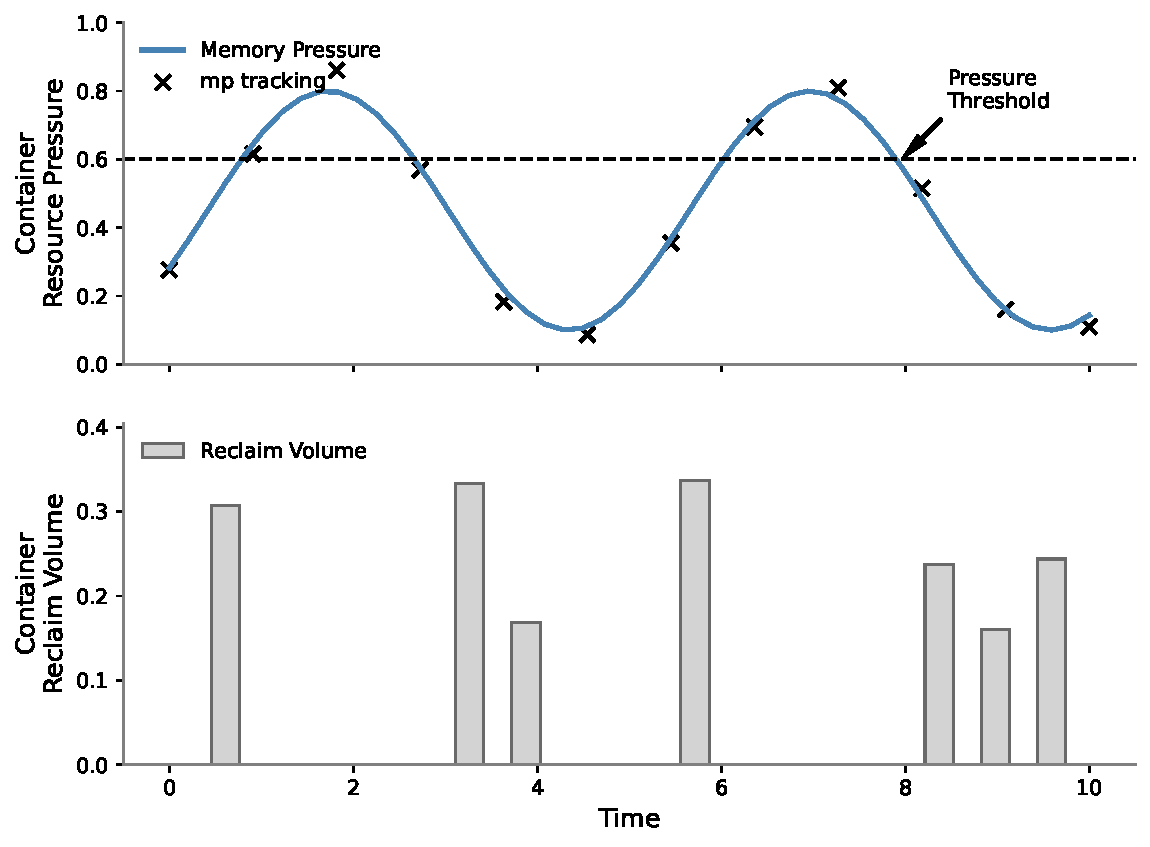
\includegraphics[width=\textwidth]{压力与回收.pdf}
\caption{内存压力与冷页回收的关系}
\label{fig:pressure_work_set}
\end{figure}

本框架中,系统总内存限制的计算公式如下:

\begin{equation}
    \label{eq:limit_adjust}
    Limit_{t+1} = 
    \begin{cases}
    Limit_t \times \left(1 + \min\left(\left(\frac{P_{actual}}{P_{target} \times C_{backoff}}\right)^2 \times M_{backoff}, M_{backoff}\right)\right) & \text{if } P_{actual} > P_{target} \\
    Limit_t \times \left(1 - \min\left(\left(\frac{P_{target}}{P_{actual} \times C_{probe}}\right)^2 \times M_{probe}, M_{probe}\right)\right) & \text{if } P_{actual} \leq P_{target}
    \end{cases}
    \end{equation}

其中,系统需要满足以下约束条件:

公式 (\ref{eq:limit_adjust}) 中的各变量含义如下:
\begin{itemize}
    \item \(Limit_{min}\):最小内存限制 (min\_size)。
    \item \(Limit_{max}\):最大内存限制 (max\_size)。
    \item \(Limit_t\):时刻 \(t\) 的内存限制。
    \item \(Limit_{t+1}\):下一时刻 (\(t+1\)) 的内存限制。
    \item \(P_{target}\):目标内存压力值 (pressure)。
    \item \(P_{actual}\):实际观察到的内存压力积分 (integral)。
    \item \(C_{probe}\):探测系数 (coeff\_probe)。
    \item \(M_{probe}\):最大探测比例 (max\_probe)。
    \item \(C_{backoff}\):退避系数 (coeff\_backoff)。
    \item \(M_{backoff}\):最大退避比例 (max\_backoff)。
\end{itemize}

该算法具有以下特点:

平方关系: 使用平方关系使得调整过程更加平滑。
最大调整限制: 设置最大调整幅度,防止内存限制的过度波动。
动态调整幅度: 根据实际压力与目标压力的偏差大小,动态调整内存限制的幅度。
非对称调整: 内存限制的增加和减少采用不同的参数。当内存不足时,可以快速增加内存限制;当内存充足时,则缓慢减少内存限制,以避免频繁的调整。
需要强调的是,公式 (\ref{eq:limit_adjust}) 只是一个示例。由于本框架部署在用户态,因此可以根据不同的应用程序、不同的应用场景和不同的服务等级目标(SLO)灵活地调整工作集估计算法。例如,对于离线分析任务,可以设置较大的目标内存压力;而对于在线分析任务,为了保证 SLO,可以设置较小的目标内存压力。



\subsection{内存压力文件系统的实现}
\label{sec:mpfs_implementation}

为了实现用户态与内核态之间的高效通信,本节主要基于 Linux 内核提供的 proc 伪文件系统(procfs)构建了一个名为 \texttt{mpfs} 的内存压力文件系统。本节将首先介绍 proc 文件系统的基本概念和特性,然后详细阐述 \texttt{mpfs} 的设计与实现细节。

\subsubsection{proc 文件系统概述}

proc 文件系统是一种特殊的、由内核动态生成的伪文件系统,通常挂载于 \texttt{/proc} 目录。它并不存储在物理磁盘上,而是存在于内存中,为用户空间提供了一种访问和修改内核信息的标准接口。proc 文件系统具有以下几个关键特性:

\begin{itemize}
    \item \textbf{动态性:} proc 文件系统中的文件和目录并非静态存在,而是由内核根据当前系统状态动态生成。
    \item \textbf{虚拟性:} proc 文件系统中的文件不占用实际的磁盘空间,它们只是内核数据的虚拟表示。
    \item \textbf{交互性:} 用户可以通过标准的文件 I/O 操作(如 \texttt{read}、\texttt{write}、\texttt{poll} 等)与 proc 文件系统中的文件进行交互,从而读取内核信息或修改内核参数。
    \item \textbf{通用性:} proc 文件系统提供了一套统一的接口,使得用户空间的应用程序无需了解内核内部的复杂数据结构,即可方便地访问内核信息。
\end{itemize}

基于 proc 文件系统的这些特性,它非常适合作为用户态与内核态之间进行信息交换的桥梁。

\subsubsection{mpfs 的设计与实现}

\texttt{mpfs} 的设计目标是提供一个轻量级、响应及时的接口,供用户态程序获取和监控系统的内存压力信息,并支持基于内存压力的事件通知机制。为了实现这一目标,\texttt{mpfs} 提供了以下三个文件接口:

\begin{itemize}
    \item \texttt{/proc/mpfs/mem\_pressure}:用于读取当前系统的内存压力值(百分比)。该文件支持 \texttt{poll} 系统调用,当内存压力超过预设阈值时,会触发可读事件,从而通知等待中的用户态程序。
    \item \texttt{/proc/mpfs/period}:用于读取和设置内存压力采样周期(单位:秒)。用户态程序可以通过写入该文件来动态调整采样频率。
    \item \texttt{/proc/mpfs/mthreshold}:用于读取和设置内存压力阈值(百分比)。当内存压力超过该阈值时,\texttt{/proc/mpfs/mem\_pressure} 文件的 \texttt{poll} 调用会返回可读事件。
\end{itemize}

表 \ref{tab:mpfs_files} 总结了 \texttt{mpfs} 中各个文件接口及其对应的文件操作函数。

\begin{table}[H]
    \centering
    \caption{\texttt{mpfs} 文件接口及操作}
    \label{tab:mpfs_files}
    \begin{tabular}{cccc} % 四列,都居中对齐
        \toprule
        \textbf{操作} & \textbf{\texttt{/proc/mpfs/mem\_pressure}} & \textbf{\texttt{/proc/mpfs/period}} & \textbf{\texttt{/proc/mpfs/mthreshold}} \\
        \midrule
        \texttt{read} & 获取内存压力 & 获取采样周期 & 获取压力阈值 \\
        \texttt{write} & -- & 设置采样周期 & 设置压力阈值 \\
        \texttt{poll} & 内存压力事件通知 & -- & -- \\
        \bottomrule
    \end{tabular}
\end{table}


\texttt{mpfs} 的核心实现基于内核模块机制。在模块初始化函数 (\texttt{mempressure\_init}) 中,通过 \texttt{proc\_create} 函数创建了上述三个文件节点,并分别指定了它们的文件操作函数集(\texttt{file\_operations} 结构)。

\begin{itemize}
    \item \textbf{\texttt{mem\_pressure}} 文件:
    \begin{itemize}
        \item \texttt{read} 操作:调用 \texttt{mempressure\_read} 函数,从全局静态变量处获取当前内存压力值,并将其格式化为字符串后复制到用户空间缓冲区。
        \item \texttt{poll} 操作:调用 \texttt{mempressure\_poll} 函数,该函数首先将当前进程添加到等待队列 \texttt{mem\_waitq} 中,然后调用\texttt{mempressure\_read}查看内存压力,。如果内存压力超过阈值,则返回 \texttt{POLLIN | POLLRDNORM},表示文件可读;否则,进程将进入睡眠状态,等待被唤醒。
    \end{itemize}

\item \textbf{\texttt{period}} 文件:
    \begin{itemize}
        \item \texttt{read} 操作:调用 \texttt{mempressure\_period\_read} 函数,该函数读取全局变量 \texttt{sample\_period}(采样周期,单位:秒),并将其格式化为字符串后复制到用户空间缓冲区。
        \item \texttt{write} 操作:调用 \texttt{mempressure\_period\_write} 函数,该函数从用户空间缓冲区读取新的采样周期值,并进行合法性检查(必须为正整数)。然后更新采样周期,等到之后工作队列就可以采用新的采样周期。
    \end{itemize}

    \item \textbf{\texttt{mthreshold}} 文件:
    \begin{itemize}
    \item \texttt{read} 操作:调用 \texttt{mempressure\_threshold\_read} 函数,该函数读取全局变量 \texttt{mem\_pressure\_threshold}(内存压力阈值,百分比),并将其格式化为字符串后复制到用户空间缓冲区。
    \item \texttt{write} 操作:调用 \texttt{mempressure\_threshold\_write} 函数,该函数从用户空间缓冲区读取新的阈值,并进行合法性检查)。然后更新阈值就可以返回。
    \end{itemize}
\end{itemize}

内存压力的周期性监测和事件通知由工作队列 \texttt{pressure\_work} 实现。工作队列的处理函数 \texttt{mempressure\_workfunc} 执行以下操作:

\begin{enumerate}
    \item 获取系统内存信息(总内存、可用内存),计算内存使用率(百分比)。
    \item 将计算得到的内存使用率更新到原子变量 \texttt{current\_usage\_percent}。
    \item 检查内存使用率是否超过阈值 \texttt{mem\_pressure\_threshold}。如果超过,则设置内存压力标志 \texttt{pressure\_flag},并通过 \texttt{wake\_up\_interruptible} 函数唤醒等待队列 \texttt{mem\_waitq} 上的所有进程。
    \item 根据当前采样周期 \texttt{sample\_period} 重新调度工作队列 \texttt{pressure\_work}。
\end{enumerate}

通过上述设计和实现,\texttt{mpfs} 为用户态程序提供了一个简洁、高效的接口,用于实时监控系统内存压力,并根据需要调整采样周期和阈值。





\section{本章小结}